
\section{Introduction}
\subsection{Motivations}
\frame
{
  \frametitle{Motivations}
%  \framesubtitle{Jean-Marc - 10 to 15 minutes}
\begin{block}{Scientific context}
\begin{itemize}
\item Complex parallel/distributed programs
\item Potentially large size parallel applications.
\item Executing on large size parallel systems:
\begin{itemize}
\item Distributed systems
\item Clusters and Grids 
\item  Desktop grids, P2P systems...
\end{itemize}
\end{itemize}
\end{block}
\begin{block}{Keypoints}
\begin{itemize}
\item Distributed heterogeneous resources
\item Dynamicity of the architecture
\item Scalability (huge amount of data)
\end{itemize}
\end{block}
%  \begin{itemize}
%  \item The institutions involved (UFRGS/UFSM/Grenoble/...)
%  \item The French-Brazilian collaboration in the domain
%  \item The importance of the visualization of parallel applications performance
%  \item The tutorial outline
%  \end{itemize}
}
\begin{frame}
\frametitle{General Objective}
\begin{block}{Help users find performance errors:}
\begin{itemize}
\item Visualization of parallelism, identify synchronization overheads,\\
\item Usage of resources, identify bottlenecks, \\
\item Behavior analysis method.
\end{itemize}
\end{block}
\pause
\begin{block}{Based on:}
\begin{itemize}
\item Execution model : user events,\\
\item Infrastructure model : Measurement environment\\
\item Visualisation model : graphical objects.
\end{itemize}
\end{block}
\end{frame}

\begin{frame}
\frametitle{Visualization of parallel program execution}
\begin{block}{Who ?}
 Program designer, 
 Program certifier, $\cdots$\\
\hfill $\cdots$ Parallel programs vendors
\end{block}
\pause
\begin{block}{Why ?}
\begin{itemize}
\item  Program debugging,  
\item Quantitative debugging (performance evaluation), 
\item Dimensionning and performance tuning
\end{itemize}
\end{block}
\pause
\begin{block}{How ? }
\begin{itemize}
\item Graphical representation of the parallel execution
\item Interactive representation (exploration)\\
- zoom in and out on time, infrastructure, on objects\\
- compute statistics
\end{itemize}
\end{block}
\end{frame}
\begin{frame}
\frametitle{Methodology}
\begin{block}{Execution model}
\begin{itemize}
\item Abstraction of the parallel execution : state / event model
\item Observability of states / Practical interest of states
\item Quality of observation (interaction tracer/application)
\end{itemize}
\end{block}
\begin{block}{Environment model}
\begin{itemize}
\item Structured set of resources (architecture)
\item Model of time : Datation model

\end{itemize}
\end{block}
\alert{\textbf{$\Rightarrow$ Manipulation language of resources, states and events}}
\end{frame}
\begin{frame}

\frametitle{Collaboration (a not so short story)}
\begin{center}\large{UFSM, UFRGS, U. of Grenoble, INRIA}\end{center}
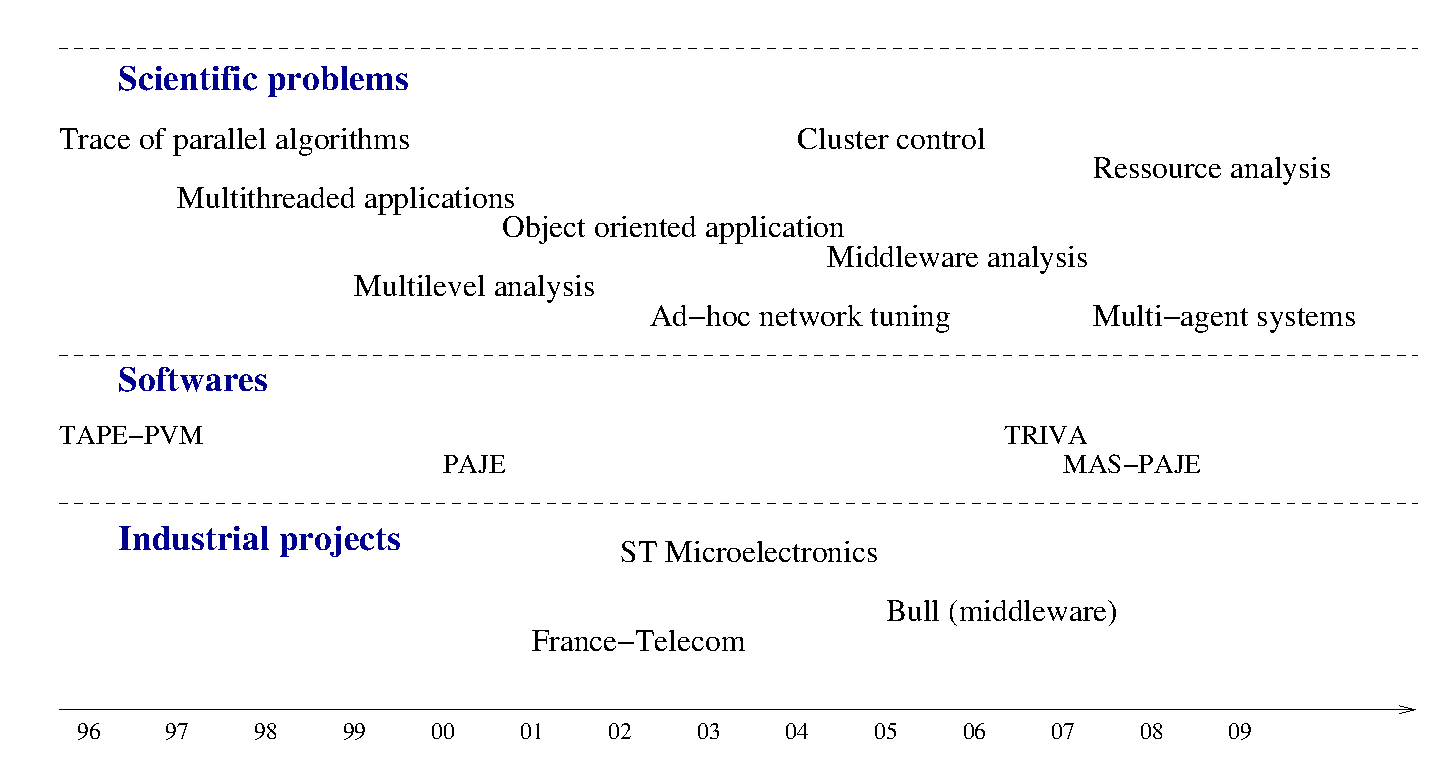
\includegraphics[width=1.1\textwidth]{img/collaboration.pdf}
\end{frame}


\frame{
  \frametitle{Introduction - Existing Tools/Techniques}
  \begin{itemize}
  \item Statistical Techniques
     \begin{itemize}
     \item ParaGraph (1990) -- bar charts, utilization Count
     \item Pablo (1993) -- bar charts + 3D scatter plot
     \item Paradyn (1995) -- histograms
     \end{itemize}
  \item Behavioral Techniques
     \begin{itemize}
     \item ParaGraph (1990) -- Gantt-chart
     \item Vampir (1996) -- time-line system view
     \item Jumpshot (1999), Paj\'e (2000) -- space-time
     \item Virtue (1999) -- virtual reality to performance analysis
     \item Kojak, ParaProf (2003) -- Call Graph
     \end{itemize}
  \item Structural Techniques
     \begin{itemize}
     \item ParaGraph (1990) -- network display / hypercube
     \item Cray Apprentice (2007) -- tree view of imbalances
     \end{itemize}
  \end{itemize}
}


\begin{frame}
\frametitle{Main difficulty}
\centerline{\alert{\large{\textbf{Large scale systems}}}}
\begin{itemize}
\item Large number of objects
\item Complexity of views
\item Level of abstraction
\item Dynamicity of the observed infrastructure

\end{itemize}
\end{frame}
\subsection{Examples}
\begin{frame}
\frametitle{Multithreaded Applications (1999)}
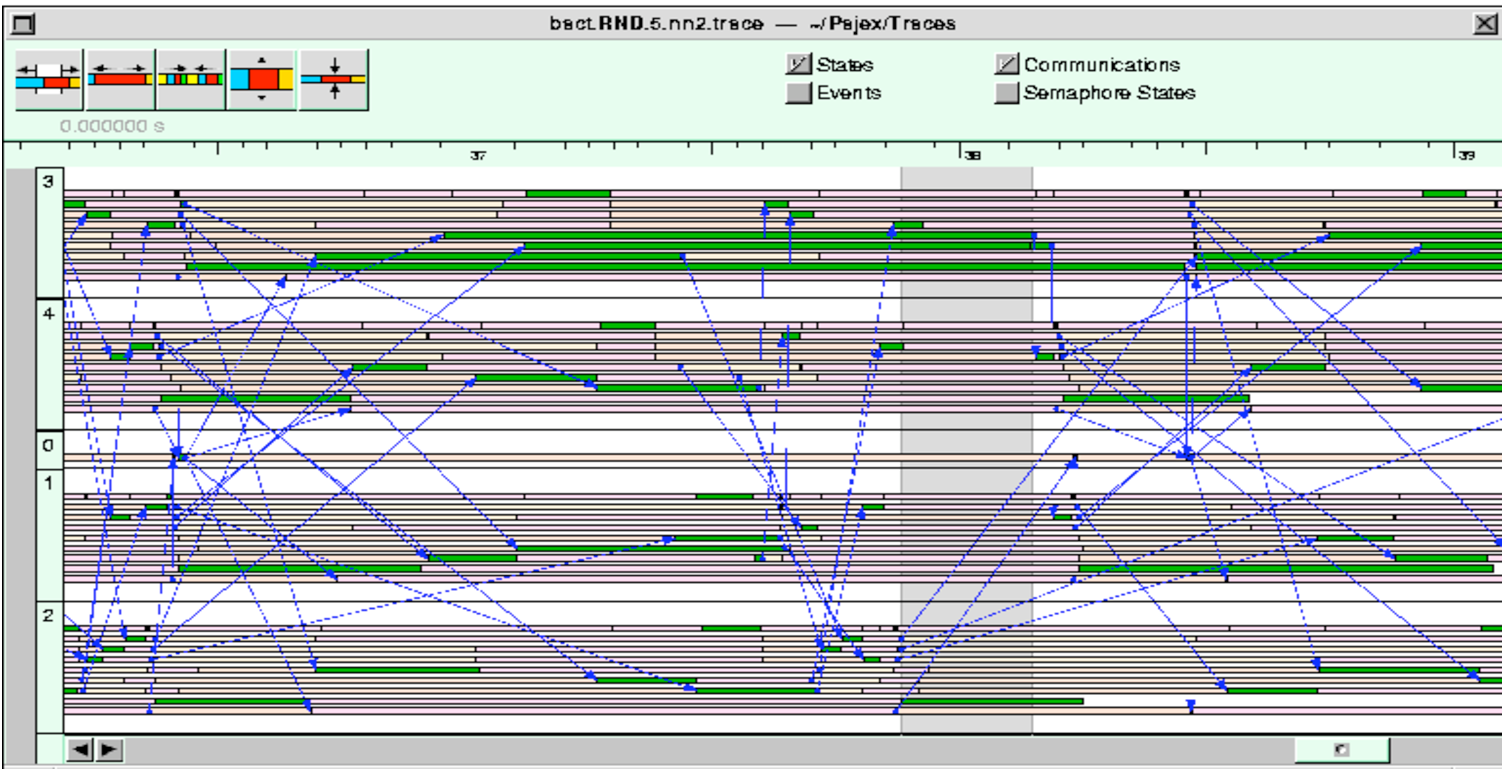
\includegraphics[width=\textwidth]{figures/Multithreaded.pdf}

\end{frame}

\begin{frame}
\frametitle{Distributed Middleware}
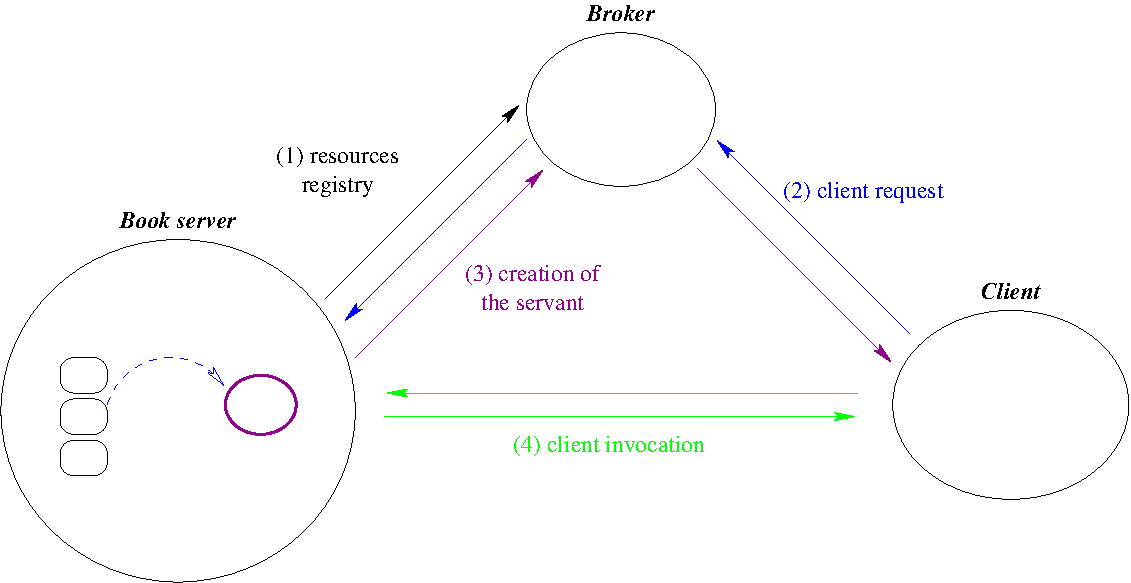
\includegraphics[width=\textwidth]{figures/ArchiTraderServerClient.pdf}
\end{frame}

\begin{frame}
\frametitle{Distributed Middleware (2)}
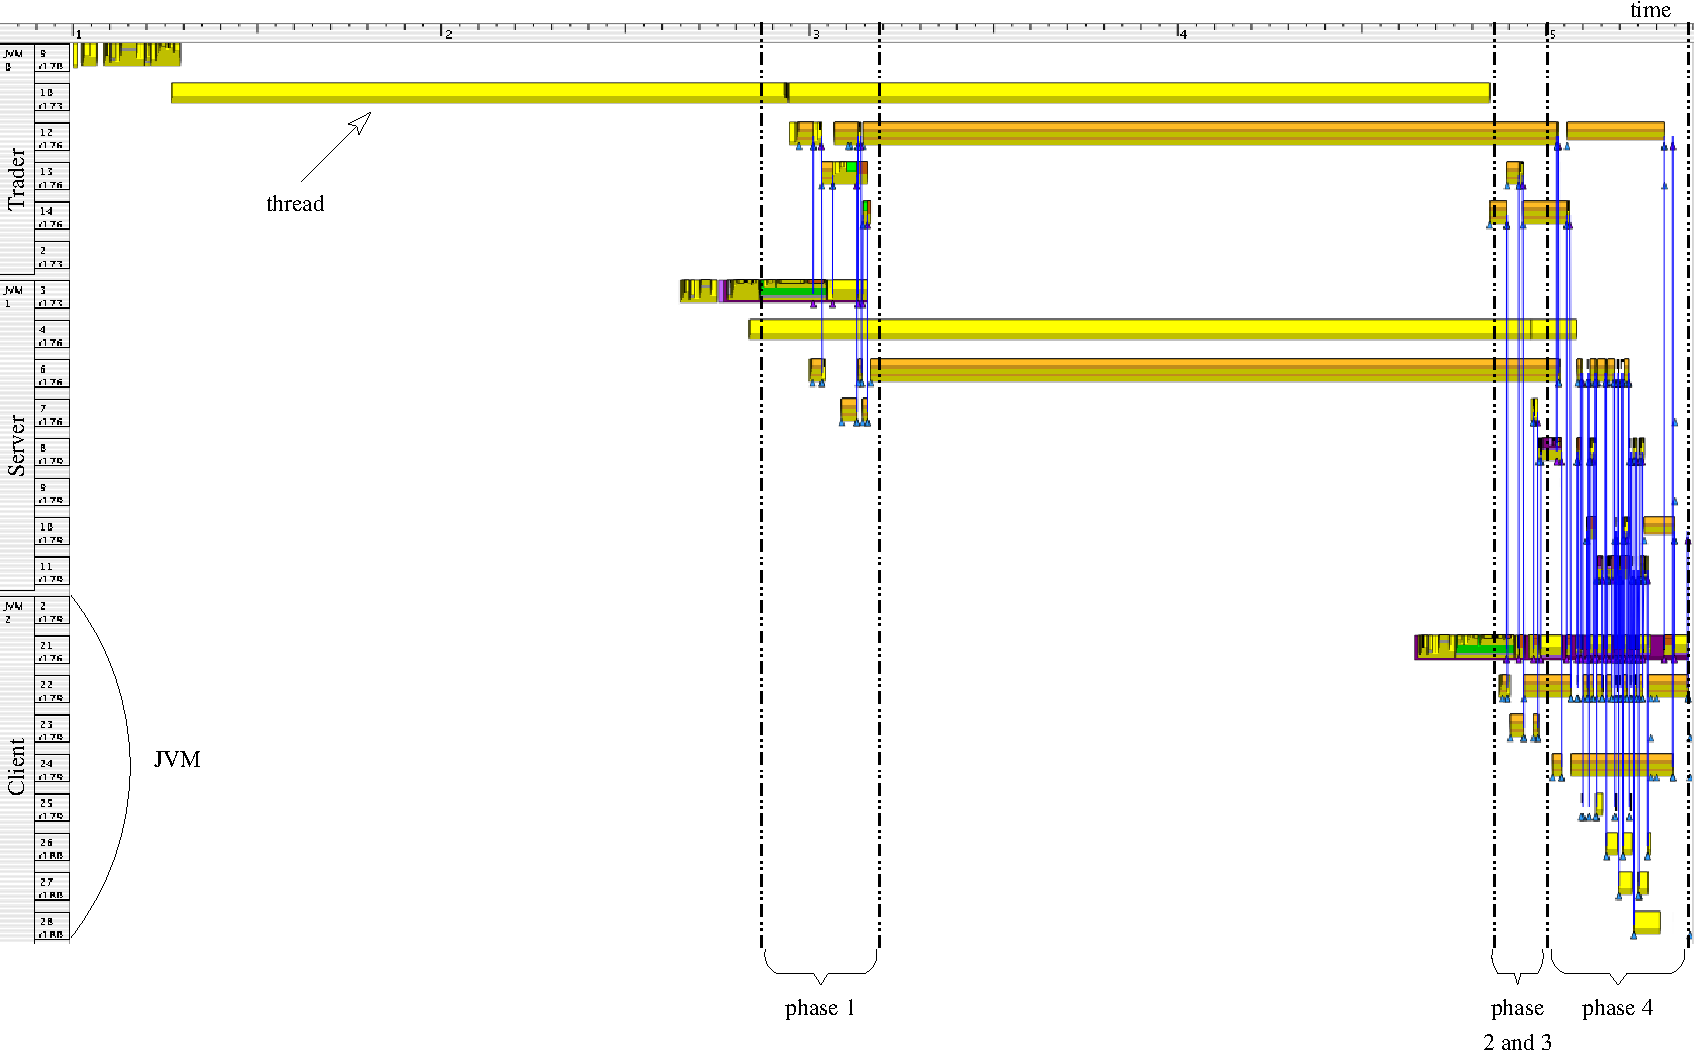
\includegraphics[width=\textwidth]{figures/Book.pdf}
\end{frame}

\begin{frame}
\frametitle{Distributed Middleware (3)}
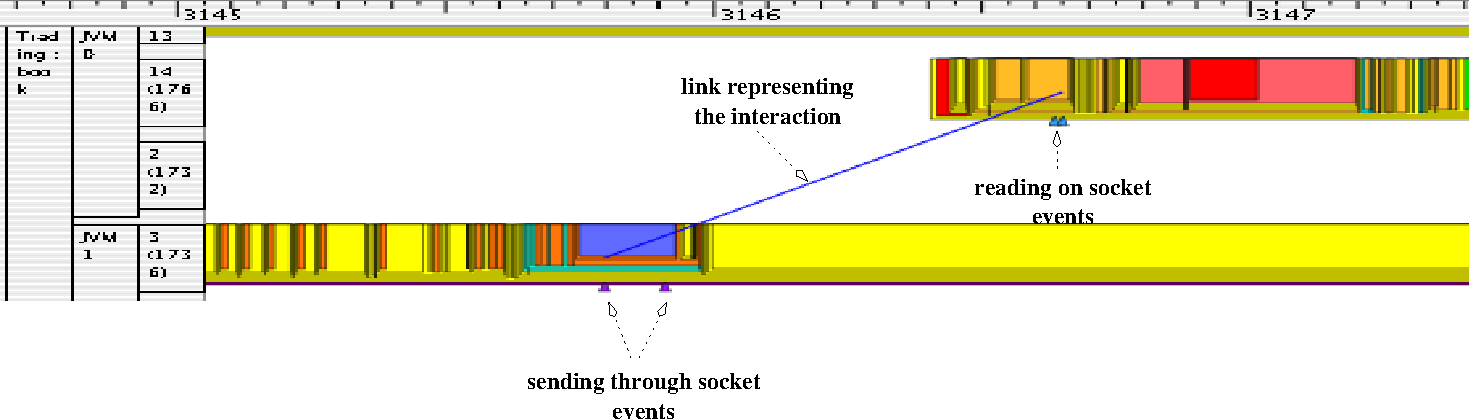
\includegraphics[width=\textwidth]{figures/RepCommPaje.pdf}
\end{frame}
\begin{frame}
\frametitle{Distributed Middleware (4)}
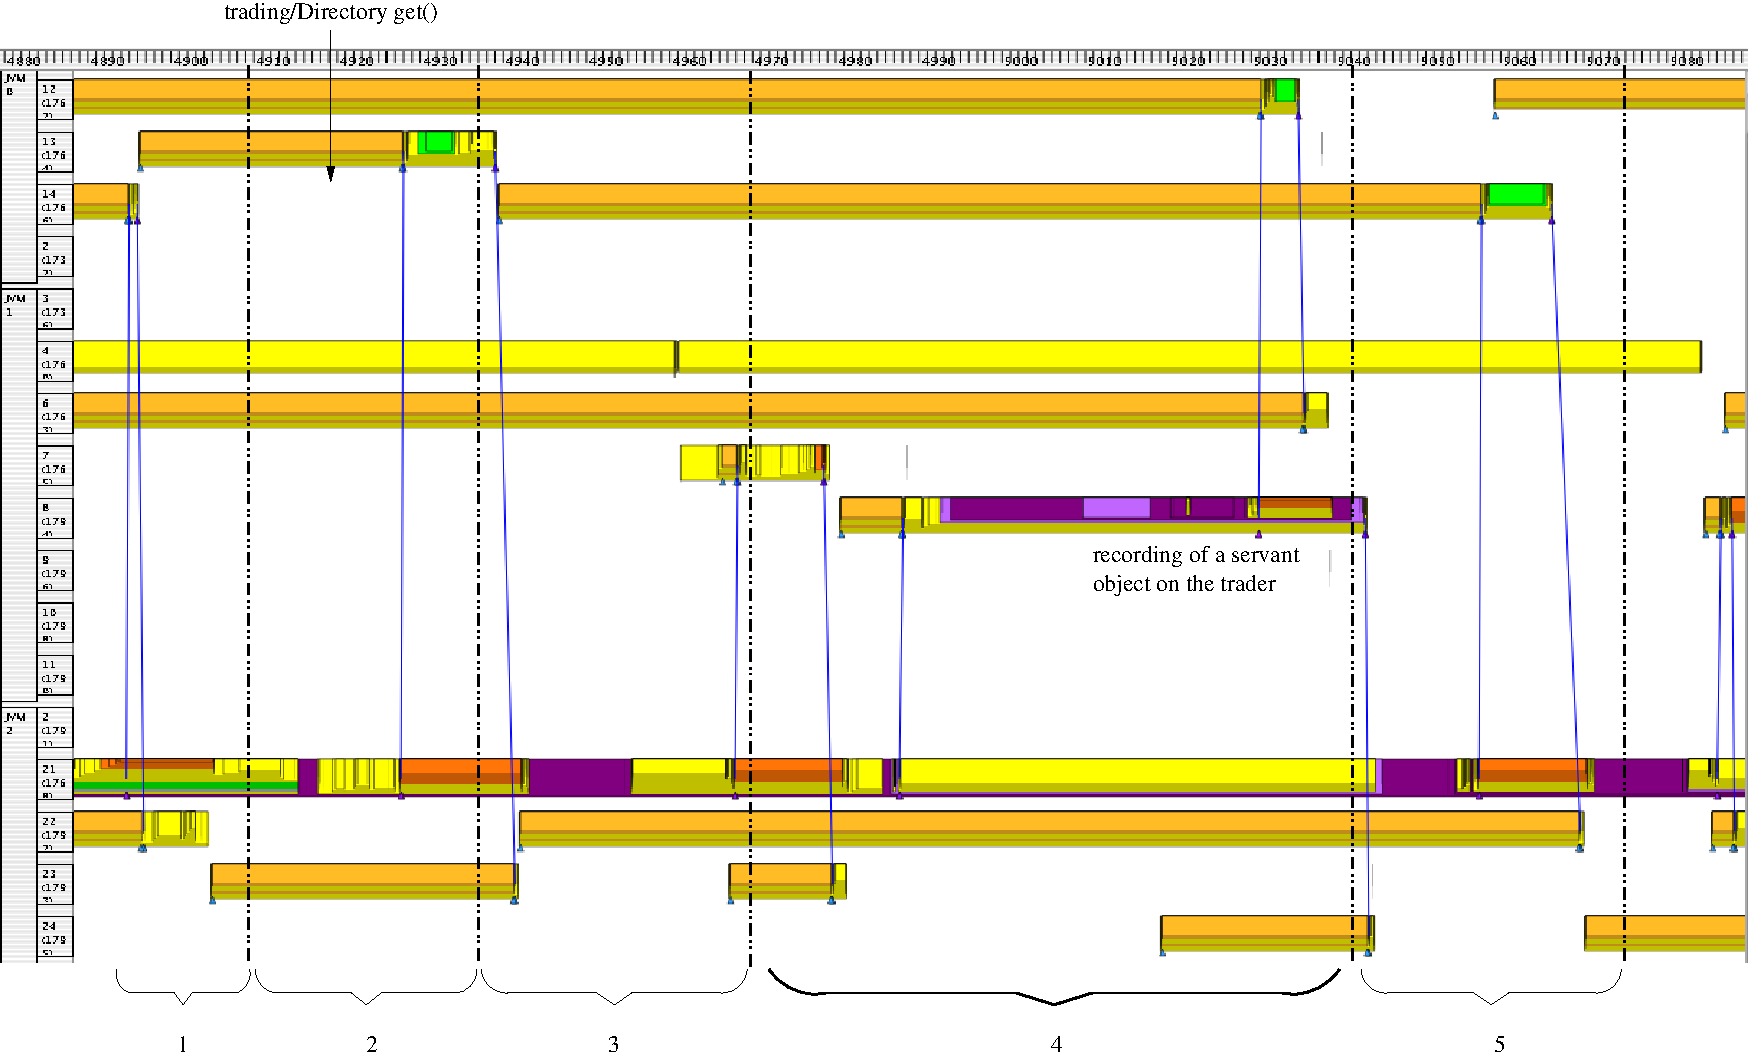
\includegraphics[width=\textwidth]{figures/Book-2.pdf}
\end{frame}
\begin{frame}
\frametitle{Distributed Middleware (5)}
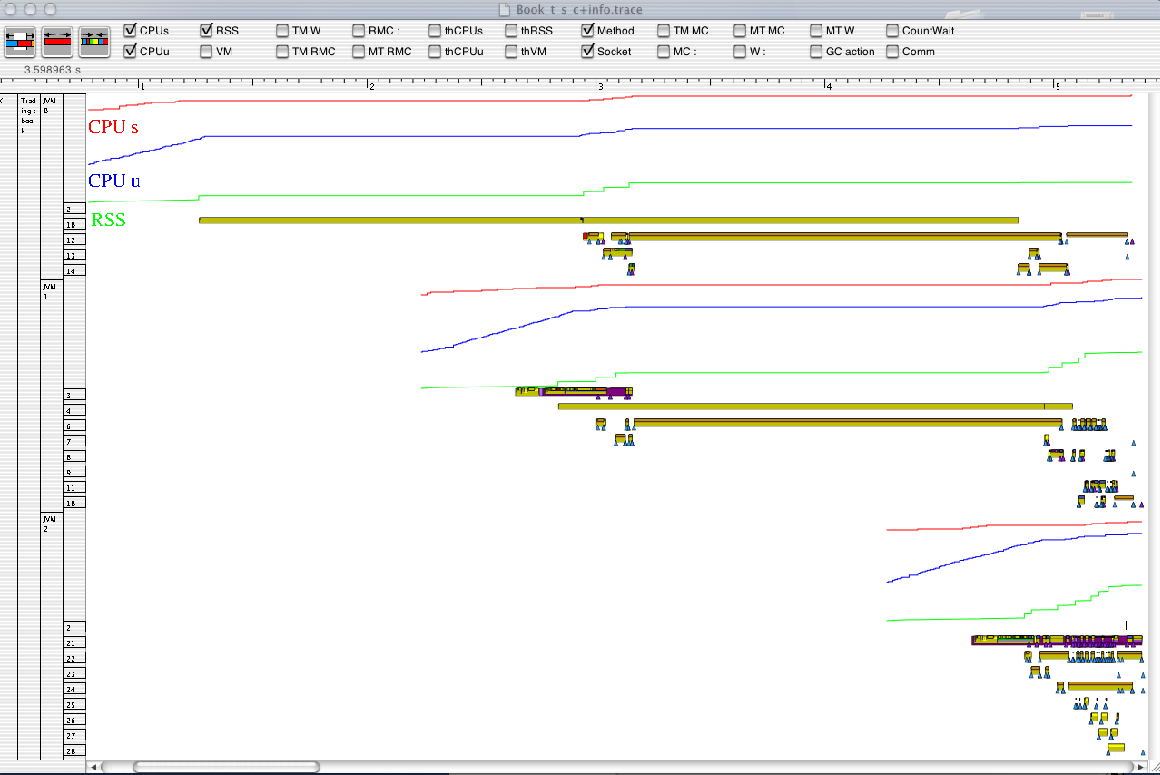
\includegraphics[width=\textwidth]{figures/BookInfoSys.pdf}

\end{frame}
\begin{frame}
\frametitle{Consensus in ad-hoc networks}
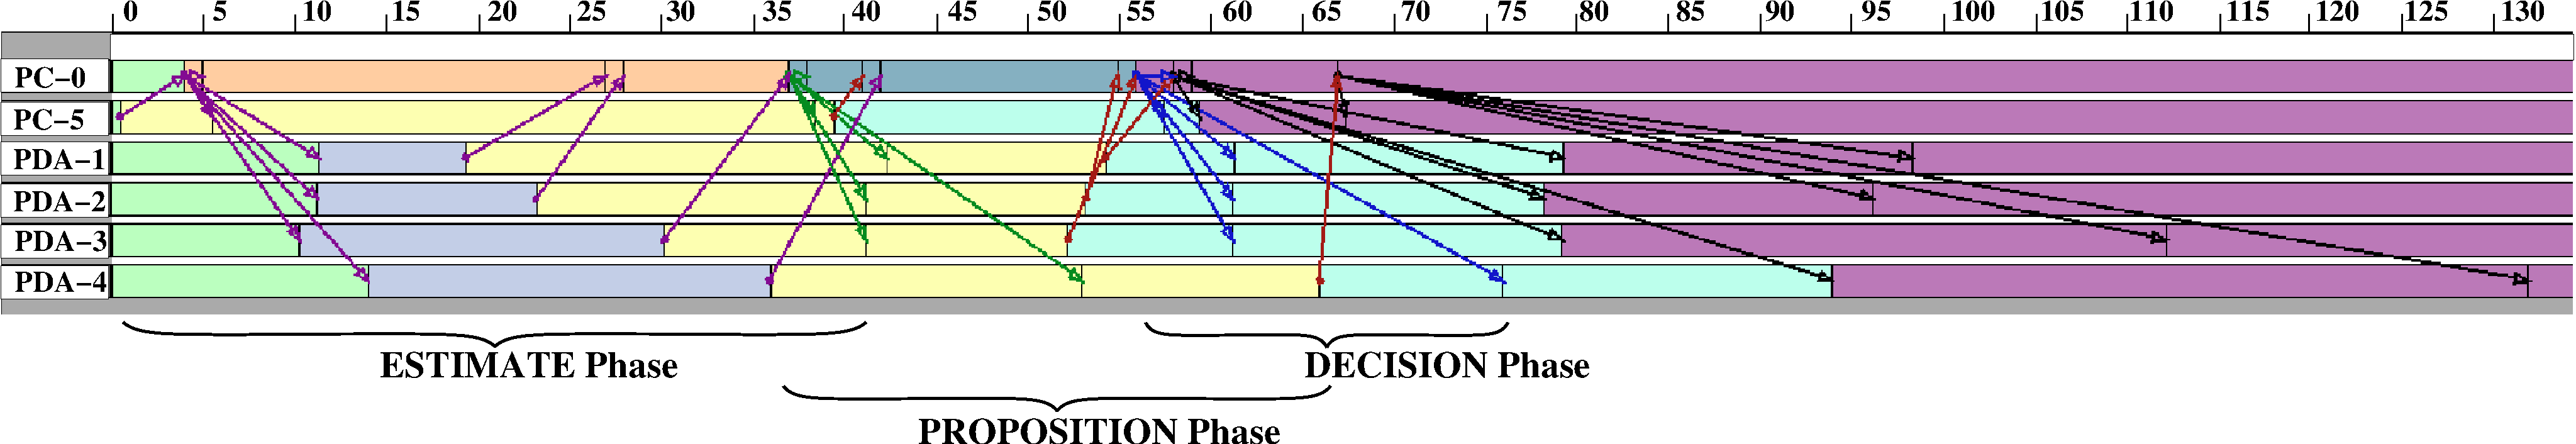
\includegraphics[width=\textwidth]{figures/Consensus1.pdf}
~\\
~\\
~\\
\pause
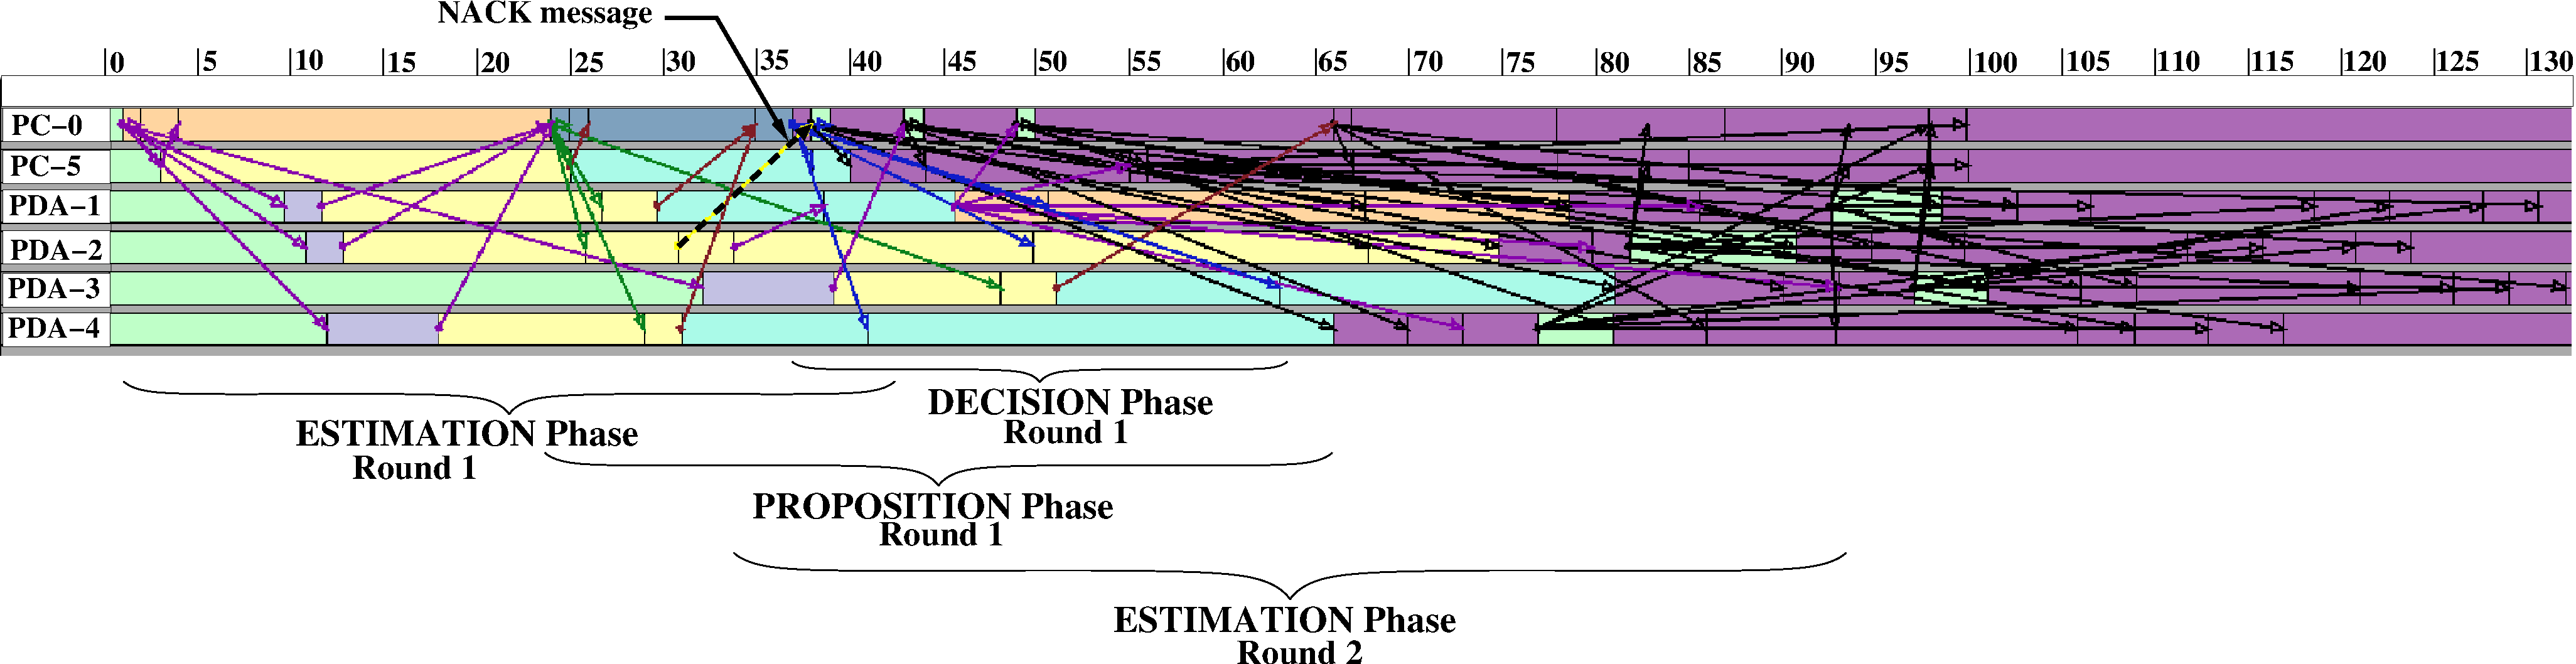
\includegraphics[width=\textwidth]{figures/Consensus2.pdf}

\end{frame}


\begin{frame}
\frametitle{Coordinator Crashes}

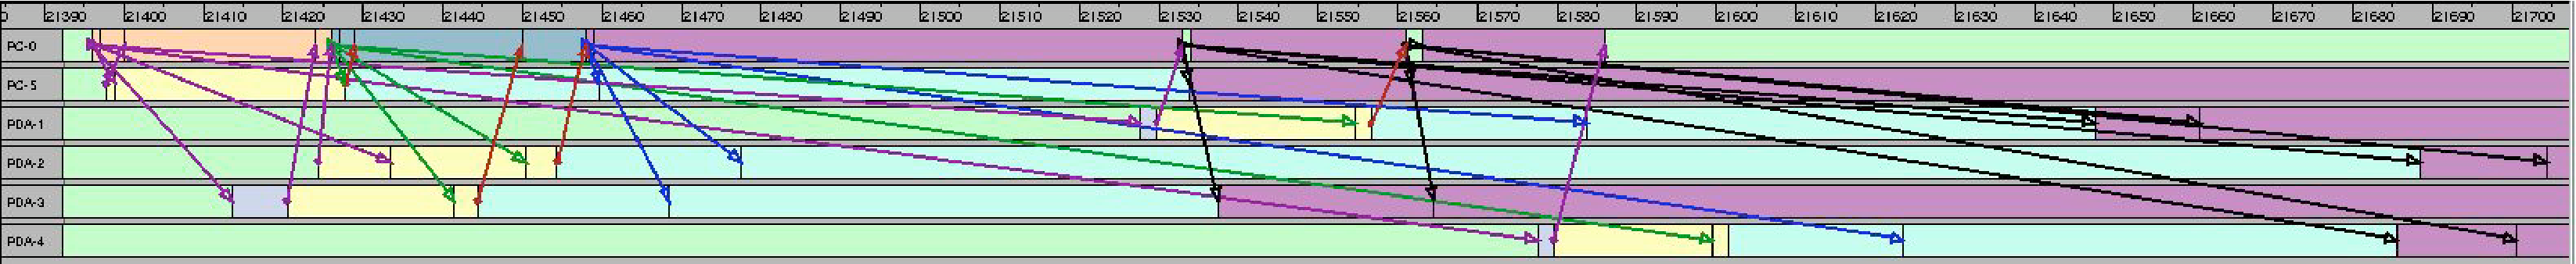
\includegraphics[width=\textwidth]{figures/trace3a.pdf}
~\\
~\\
~\\
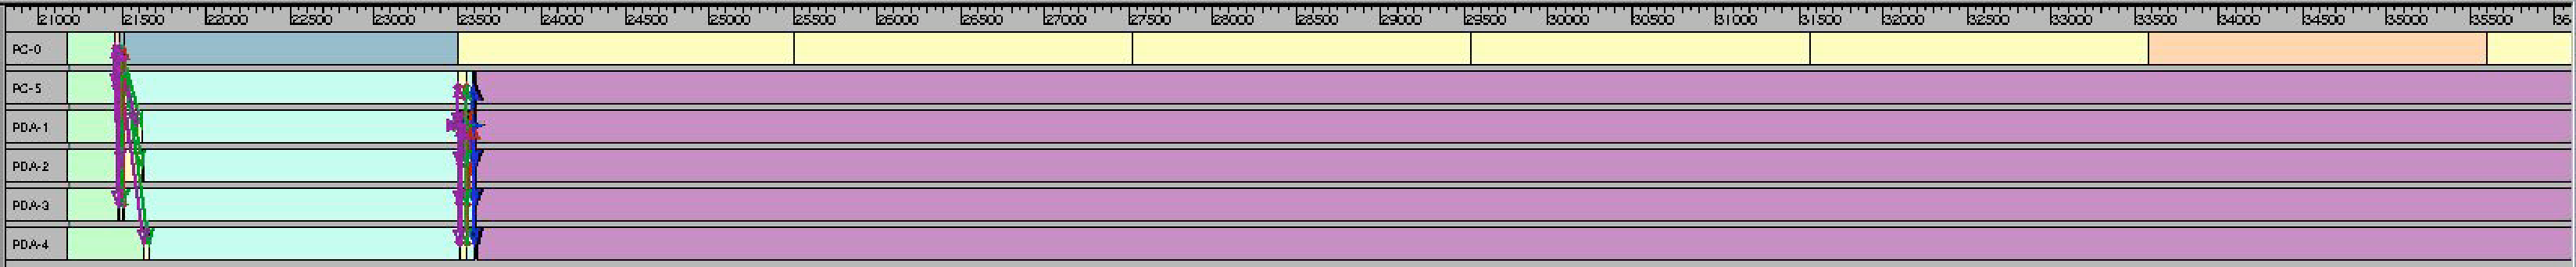
\includegraphics[width=\textwidth]{figures/trace3b.pdf}
~\\
~\\
~\\
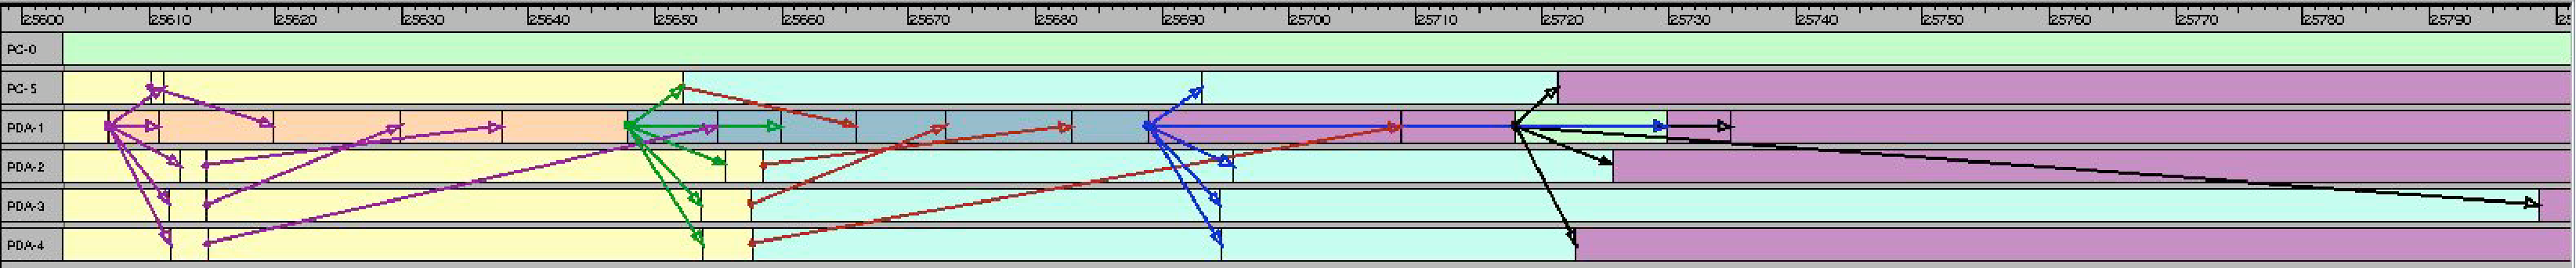
\includegraphics[width=\textwidth]{figures/trace3c.pdf}
\end{frame}

\begin{frame}
\frametitle{Multi-Agent Systems}

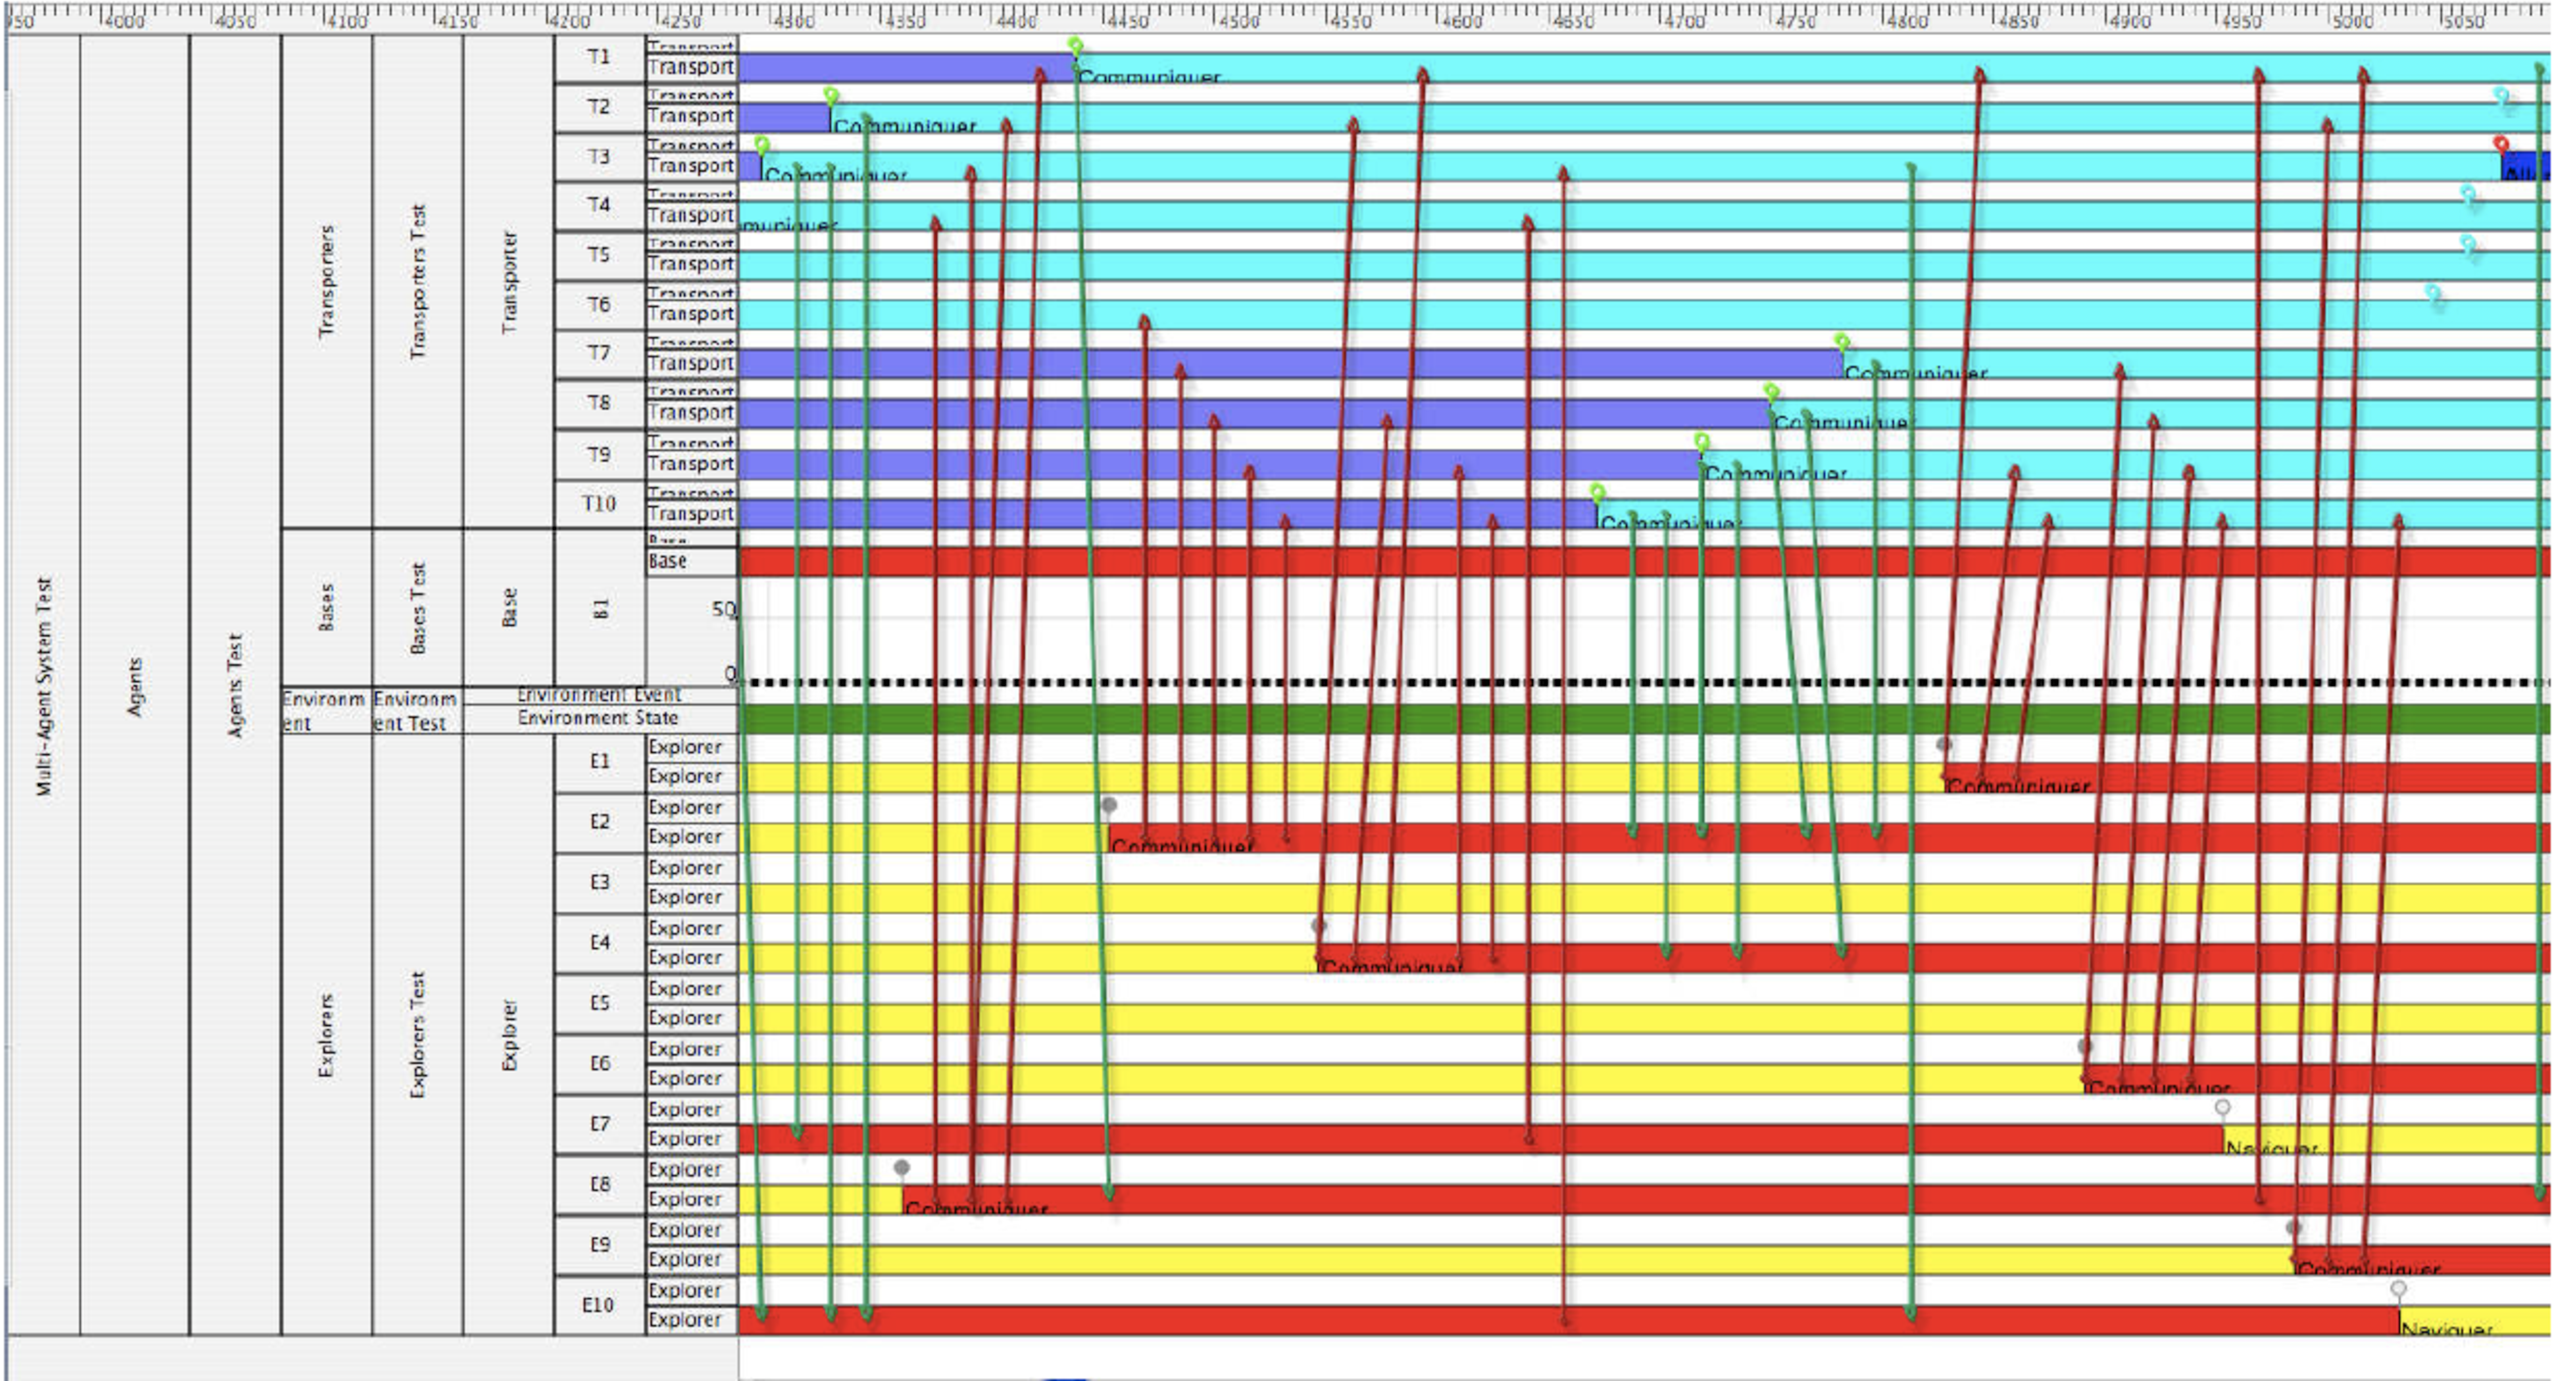
\includegraphics[width=\textwidth]{figures/SMA.pdf}

\end{frame}
%\begin{frame}
%\frametitle{ Crash and recovery}
%
%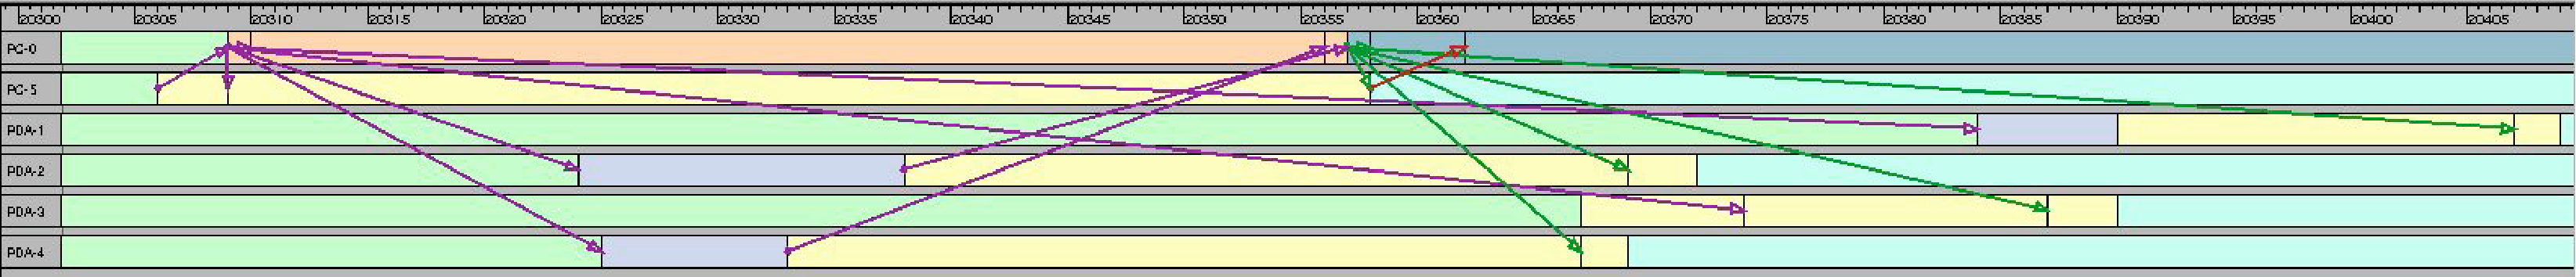
\includegraphics[width=\textwidth]{figures/trace4a.pdf}
%~\\~\\
%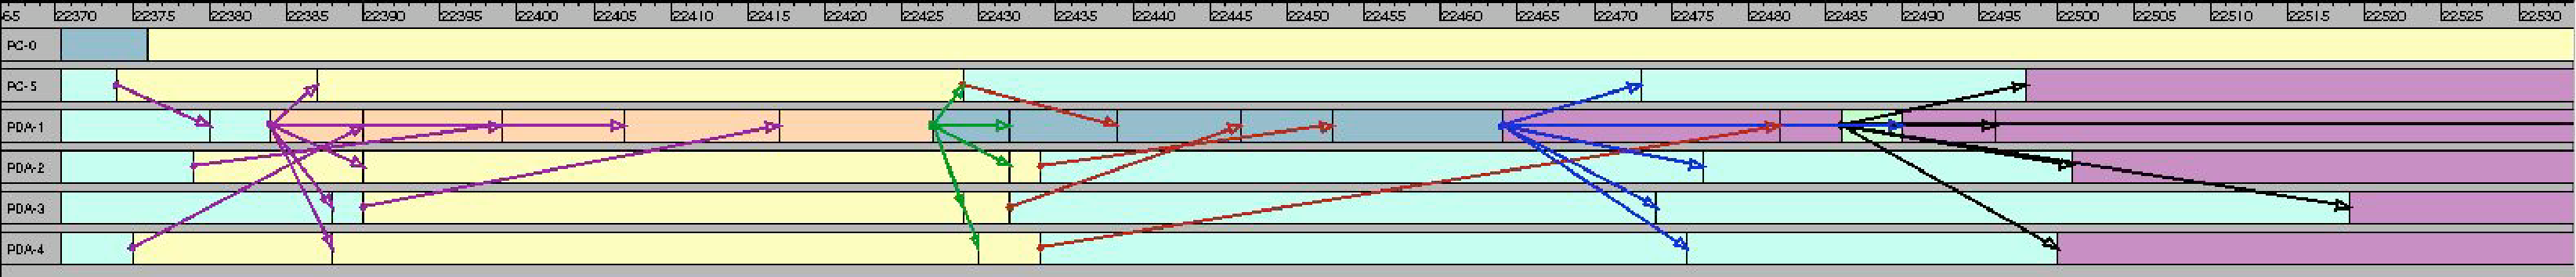
\includegraphics[width=\textwidth]{figures/trace4b.pdf}
%~\\~\\
%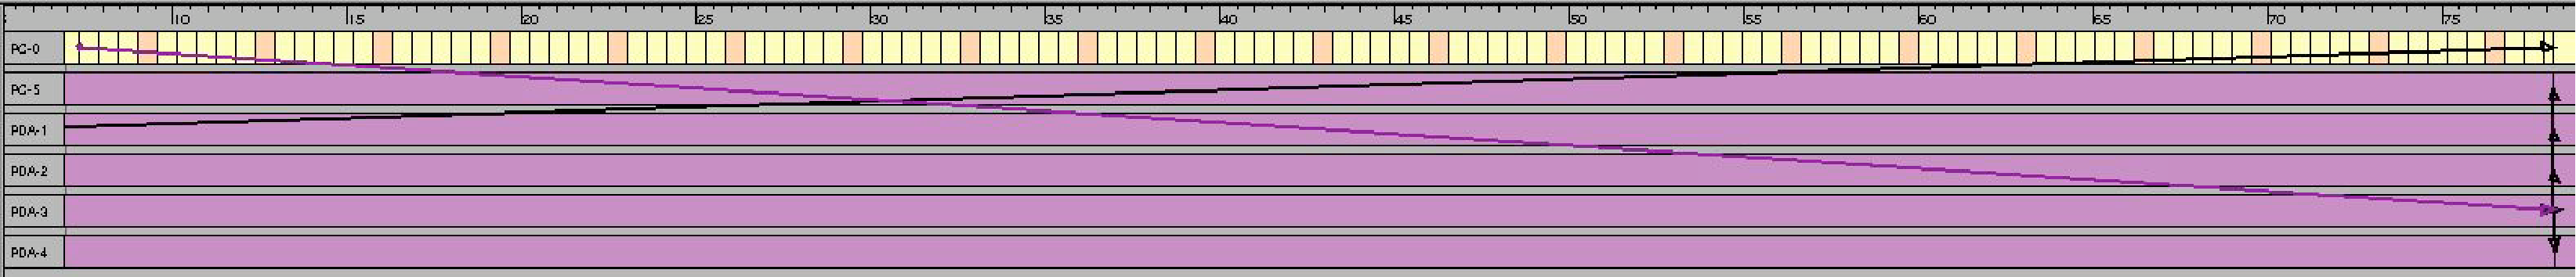
\includegraphics[width=\textwidth]{figures/trace4c.pdf}%4d
%~\\~\\
%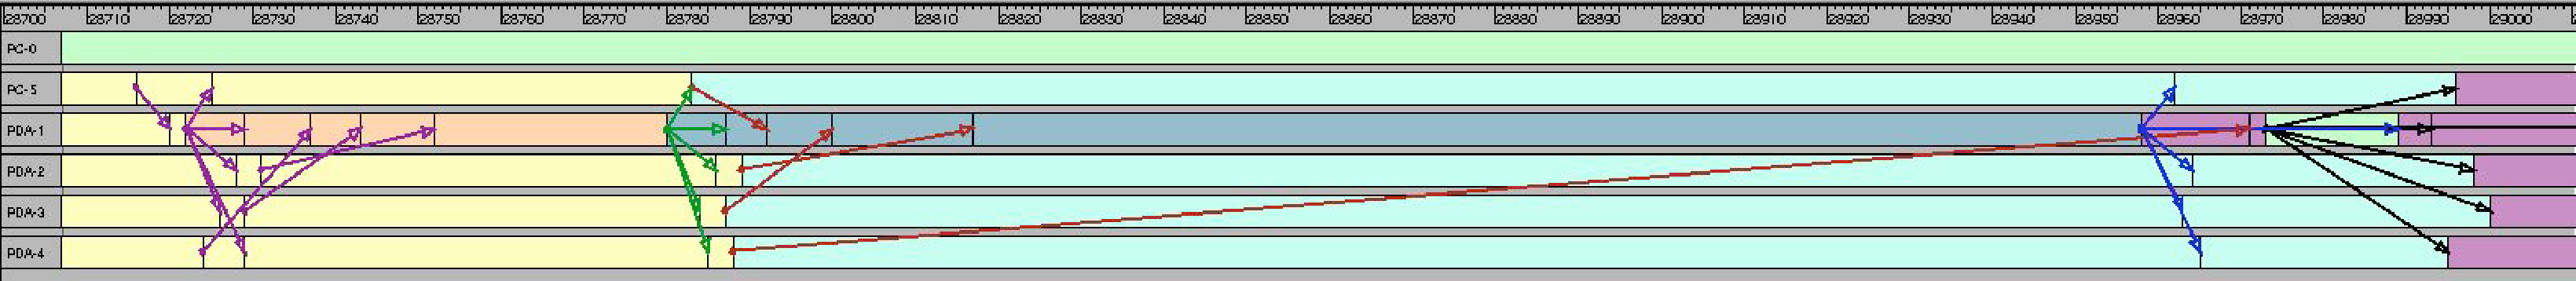
\includegraphics[width=\textwidth]{figures/trace4d.pdf}%5a
%
%\end{frame}


%\begin{frame}
%\frametitle{Sequence of crash}
%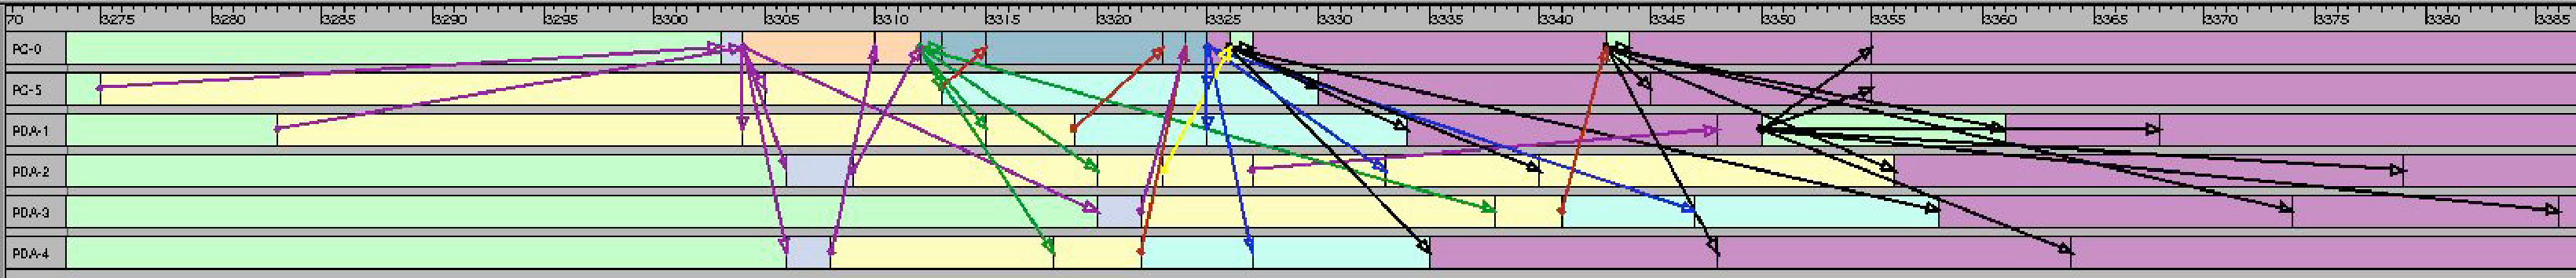
\includegraphics[width=\textwidth]{figures/trace6a.pdf}
%~\\
%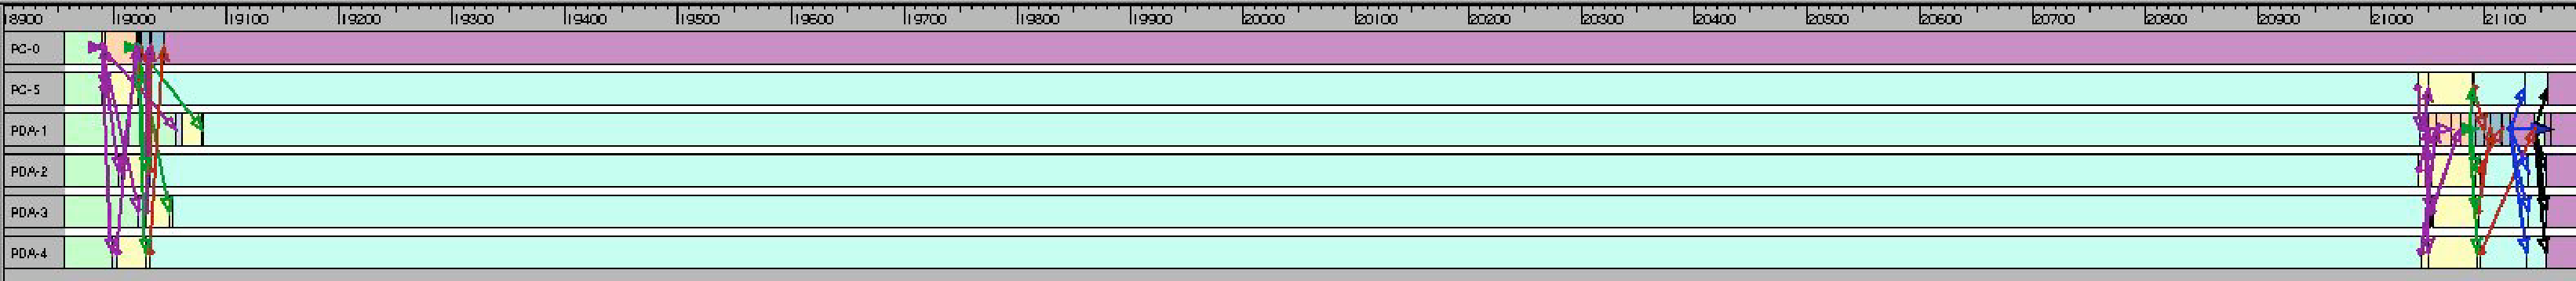
\includegraphics[width=\textwidth]{figures/trace6b.pdf}
%~\\
%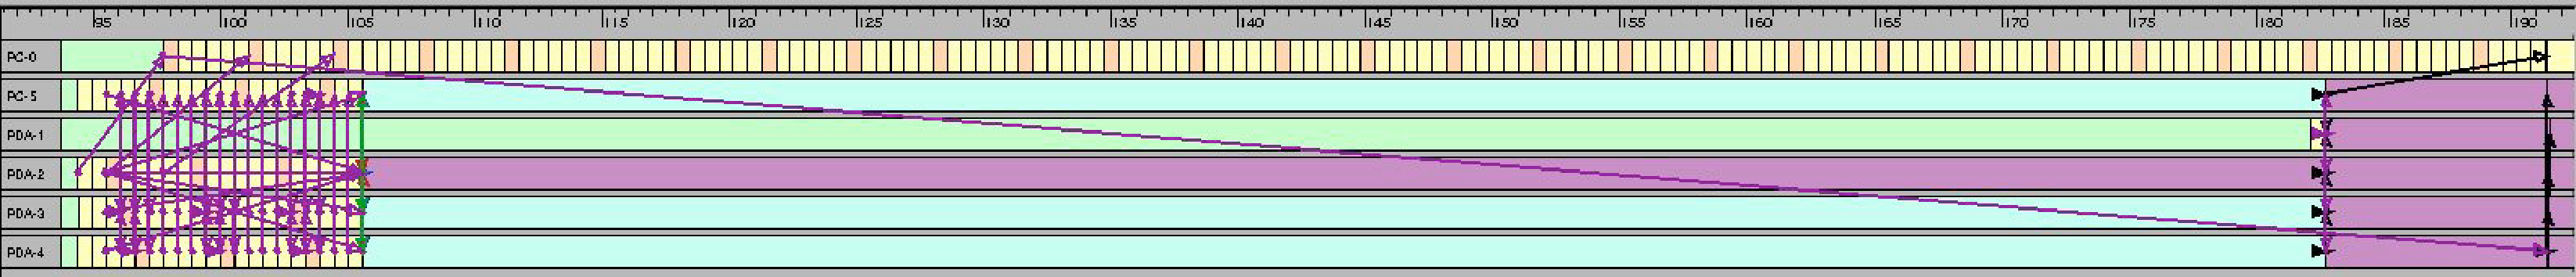
\includegraphics[width=\textwidth]{figures/trace6c.pdf}
%
%
%\end{frame}


%\begin{frame}
%\frametitle{Typical examples (use case)}
%\begin{description}
%\item Multi-threaded application : un vieux (pierre-éric) ou un kaapi 
%\item Resource usage monitoring : monitoring de grille 
%\item Ad-hoc networks (distributed protocol) : travail de Corine
%\item 
%\item Object based distributed applications : multi-niveau java
%\item Multi-agent systems : exemple paams
%\end{description}
%\end{frame}
